\section{OpenMP}

\definecolor{bostonuniversityred}{rgb}{0.8, 0.0, 0.0}
\subsection{Introdução}

\begin{frame}{OpenMP (\textit{Open Multi-Processing}) - Introdução}
	\begin{itemize}
		\item Biblioteca que fornece uma API (\textit{Application Programming Interface}) para programação paralela via memória compartilhada.
		\medskip
		\pause
		\item Já existem bibliotecas com a mesma função, como a Pthread \\(\textit{POSIX Threads Programming})\footnote{\url{http://is.gd/FJQyEr}}, por que usar a OpenMP?
		\pause
		\begin{figure}
			\centering
			 \begin{adjustwidth}{-1cm}{}
			\resizebox{\columnwidth}{!}{%
		\begin{tabular}{|c|c|c|}
			\hline
			\cellcolor{gray}{\color{white}\textbf{Requisitos}} & 
			\cellcolor{gray}{\color{white}\textbf{Pthread}} & 
			\cellcolor{gray}{\color{white}\textbf{OpenMP}}\\ \hline
			\textbf{Comportamento de cada thread\footnote{Linha de execução de uma tarefa}} &
			Programador deve especificar manualmente &
			\pbox{3cm}{\vspace{0.1 in}Compilador e sistema de\\ execução lidam\vspace{0.1 in}} \\ \hline
			\textbf{Portabilidade} & \pbox{20cm}{\vspace{0.1 in} Pode ser carregada em qualquer programa,\\ em qualquer compilador,\\ em C/C++\vspace{0.1 in}} & \pbox{20cm}{\vspace{0.1 in}Depende do suporte do\\ compilador.\\OpenMP faz a especificação e os\\ desenvolvedores dos compiladores\\ implementam\vspace{0.1 in}}\\ \hline
			\textbf{Nível de programação} & $\downarrow$ baixo nível & $\uparrow$ alto nível \\ \hline
		\end{tabular}
	}
	\caption {Pthread $\times$ OpenMP}
	 \end{adjustwidth}
		
	\end{figure}
	\end{itemize}
\end{frame}

\begin{frame}{OpenMP - Introdução}
	\begin{itemize}
		\item \textbf{Uso de funções, variáveis globais e macros\footnote{https://gcc.gnu.org/onlinedocs/cpp/Macros.html}:} Inserção do\\ cabeçalho \texttt{omp.h}.
		\pause
		\medskip
		\item Provê uma API baseada em diretivas, chamadas \texttt{pragmas}.
		\medskip
		\begin{itemize}
			\item São instruções especiais do pré-processador de C/C++
			\smallskip
			\item Permitem especificar comportamento não presente por padrão na linguagem.
			\smallskip
			\item \textbf{Portabilidade:} Se o compilador não suporta, a diretiva é ignorada.
			\smallskip
			\item São especificadas em uma linha, caso excedam adiciona-se o caractere de escape \texttt{\textbackslash} ao final da linha.
			\smallskip
			\item \textbf{Forma:} \texttt{\#pragma omp} $<$diretivas$>$.
		\end{itemize}
	\end{itemize}
\end{frame}

\begin{frame}[fragile]
%	\begin{adjustwidth}{0.2cm}{}
	\fontsize{8.5pt}{7.2}\selectfont
\begin{lstlisting}[caption=omp\_hello.c]
#include <stdio.h>
#include <stdlib.h>
#include <omp.h>
void Hello(void);

int main(int argc, char* argv[]) {
	int thread_count = strtol(argv[1], NULL, 10);

	#pragma omp parallel num_threads(thread_count)
	Hello();

	return 0;
}

void Hello(void) {
	int my_rank = omp_get_thread_num();
	int thread_count = omp_get_num_threads();

	printf("Hello from thread %d of %d\n", 
	            my_rank, thread_count);
}
	\end{lstlisting}
	\fontsize{10pt}{7.2}\selectfont	
%\end{adjustwidth}
\end{frame}

\subsection{Compilando e executando}

\begin{frame}[fragile]{OpenMP - Compilando e executando}
	\begin{itemize}
		\item Para compilar com suporte à OpenMP utilizando o \texttt{gcc}\footnote{A OpenMP é suportada no \texttt{gcc} desde a versão 4.2 $<$\url{http://is.gd/MKkNVK}$>$}, adiciona-se o parâmetro \texttt{-fopenmp}:
	\end{itemize}
	\begin{adjustwidth}{-1.6cm}{}
	\fontsize{9pt}{7.2}\selectfont
	\begin{lstlisting}[language=bash]
				$ gcc -g -Wall -fopenmp -o omp_hello omp_hello.c
	\end{lstlisting}
	\fontsize{10pt}{7.2}\selectfont
	\end{adjustwidth}
	\pause
	\begin{itemize}
		\item Executando o programa, especificando 4 \textit{threads} para execução:
	\end{itemize}
	\begin{adjustwidth}{-1.6cm}{}
	\fontsize{9pt}{7.2}\selectfont
	\begin{lstlisting}[language=bash]
				$ ./opm_hello 4
	\end{lstlisting}
	\fontsize{10pt}{7.2}\selectfont
	\end{adjustwidth}
	\pause
	\begin{itemize}
		\item Gerando uma \textbf{possível} saída:
		\medskip
		\begin{itemize}
			\item \textit{Threads} competem por acesso á saída padrão (\texttt{stdout}).
		\end{itemize}
	\end{itemize}
		\begin{adjustwidth}{-1.6cm}{}
			\fontsize{9pt}{7.2}\selectfont
			\begin{lstlisting}[language=bash]
					Hello from thread 1 of 4
					Hello from thread 2 of 4
					Hello from thread 0 of 4
					Hello from thread 3 of 4
			\end{lstlisting}
			\fontsize{10pt}{7.2}\selectfont
		\end{adjustwidth}
\end{frame}

\subsection{Checagem de Erros}

\begin{frame}[fragile]{OpenMP - Checagem de Erros}
	\begin{itemize}
		\item A diretiva \texttt{\# pragma} é ignorada por compiladores que não a suportam, porém caso o compilador não suporte a OpenMP, a diretiva \texttt{\#include <omp.h>} e chamadas de métodos como\\ \texttt{omp\_get\_thread\_num} e \texttt{omp\_get\_num\_threads} vão gerar erros.
		\pause
		\medskip
		\item É importante verificar se o compilador suporta a OpenMP, verifica-se se a macro \texttt{\_OPENMP} está definida:
		\fontsize{8pt}{7.2}\selectfont
\begin{lstlisting}
#ifdef _OPENMP
    #include <omp.h>
#endif
...
#ifdef _OPENMP
    int my_rank = omp_get_thread_num();
    int thread_count = omp_get_num_threads();
#else
    int my_rank = 0;
    int thread_count = 1;
#endif
\end{lstlisting}
\fontsize{10pt}{7.2}\selectfont
	\end{itemize}
\end{frame}

\subsection{Diretivas}

\begin{frame}{OpenMP - Diretivas}
	\begin{itemize}
		\item \texttt{\# pragma omp parallel}:
		\medskip
		\begin{itemize}
			\item Especifica que um número determinado de \textit{threads} devem executar o \textbf{bloco estruturado de código} consecutivo.
			\medskip
			\item \textbf{Bloco estruturado de código:}
			\begin{itemize}
				\item Conjunto de código com um ponto de entrada e um ponto de saída.
				\smallskip
				\item Permite invocação do comando \textbf{exit} no meio do bloco.
				\smallskip
				\item Proíbe qualquer desvio externo que entre no meio do bloco ou que saia para fora do bloco.
			\end{itemize}
			\medskip
			\begin{columns}
				\column{0.55\linewidth}
					\item Cada \textit{thread}:
					\smallskip
					\begin{itemize}
						\item É um \texttt{fork} do programa principal, compartilhando da maioria de seus recursos.
						\smallskip
						\item Possui sus própria pilha de memória e contador de programa.
						\smallskip
						\item Quando completa o trabalho, executa o \texttt{join} e se junta ao processo principal.
					\end{itemize}
					\medskip
					\item Todo esse gerenciamento de \textit{threads} é feito pela OpenMP.
				\column{0.45\linewidth}
					\begin{figure}[H]
						\centering
						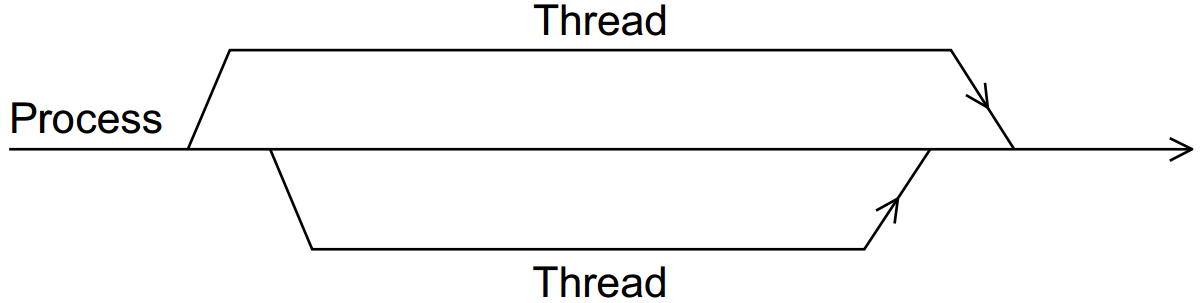
\includegraphics[width=1\linewidth]{img/OpenMP/thread}
						\caption[Fork e Join de duas threads]{\texttt{Fork} e \texttt{Join} de duas \textit{threads}}
						\label{fig:thread}
					\end{figure}
			\end{columns}
		\end{itemize}
	\end{itemize}
\end{frame}

\begin{frame}{OpenMP - Diretivas}
	\begin{itemize}
		\item \texttt{\# pragma omp parallel}:
		\medskip
		\begin{itemize}
			\item Pode ser ou não especificada a quantidade de \textit{threads} a serem executadas.
			\smallskip
			\begin{itemize}
				\item Caso não seja, é determinado em tempo de execução (uma \textit{thread} por \textit{core} disponível.)
				\smallskip
				\item Para especificar uma quantidade $n$ de \textit{threads}, usa-se: \\ \texttt{\# pragma omp parallel num\_threads(n)}
				\smallskip
				\item Alguns sistemas \textbf{podem} limitar a quantidade de \textit{threads} que podem ser executadas.
			\end{itemize}
			\medskip
			\pause
			\item Quando o compilador reconhece a diretiva \texttt{parallel}:
			\begin{itemize}
				\item A \textit{thread} do programa principal continua executando (\textbf{mestre}) e são criadas $n-1$ \textit{threads} (\textbf{escravos}) para executar o bloco de código consecutivo, formando o conjunto de $n$ \textit{threads} chamado \textbf{time}.
				\smallskip
				\item \textbf{Barreira implícita:} Se uma \textit{thread} do \textbf{time} termina a execução do bloco, espera por todas as outras \textit{threads}. Quando todas terminam, as \textit{threads} do tipo \textbf{escravo} são terminadas e o \textbf{mestre} continua executando.
			\end{itemize}
		\end{itemize}
	\end{itemize}
\end{frame}

\subsubsection{Escopo de variáveis}

\begin{frame}{Escopo de variáveis}
	\begin{itemize}
		\item Relembrando, em C/C++:
		\smallskip
		\begin{itemize}
			\item Variáveis declaradas dentro de funções, podem ser usadas apenas dentro das funções (\textbf{escopo local}).
			\smallskip
			\item Variáveis declaradas fora de qualquer função, podem ser usadas em qualquer lugar no arquivo onde foram declaradas (\textbf{escopo global}).
		\end{itemize}
		\medskip
		\pause
		\item Na especificação da OpenMP, variáveis dentro de um bloco executado pela diretiva \texttt{parallel} (pode ser acessada por todas as \textit{threads} do \textbf{time}) tem dois escopos:
		\smallskip
		\begin{enumerate}
			\item \textbf{Compartilhado:} Variáveis declaradas antes fora do bloco estruturado de código que está sendo executado em paralelo, mas que são acessíveis.
			\smallskip
			\item \textbf{Privado:} Variáveis declaradas dentro do bloco estruturado de código que está sendo executado em paralelo. Cada \textit{thread} vai ter sua própria variável declarada em sua pilha de memória.
		\end{enumerate}
	\end{itemize}
\end{frame}

\begin{frame}[fragile]{OpenMP - Diretivas}
	\begin{itemize}
		\item \texttt{\# pragma omp critical}:
		\medskip
		\item Quando múltiplas \textit{threads} tentam acessar o mesmo recurso, acontece o que é chamado de \textbf{condição de corrida}:
		\smallskip
		\begin{itemize}
			\item Se algum dos acessos for para escrita, pode resultar em inconsistência dos dados.
			\smallskip
			\item \textit{Threads} podem ler valor inválidos.
		\end{itemize}
		\medskip
		\pause
		\item O bloco de código contendo o recurso compartilhado é chamado de \textbf{sessão crítica}.
		\medskip
		\pause
		\item Quando uma \textit{thread} está dentro de uma sessão crítica, somente ela pode alterar o recurso (\textbf{exclusão mútua}).
		\medskip
		\pause
		\item Para garantir exclusão mútua à um bloco estruturado de código utilizando a OpenMP, adiciona-se a diretiva \texttt{\#pragma omp critical}
\fontsize{8pt}{7.2}\selectfont
\begin{lstlisting}
...
# pragma omp critical
altera_recurso_compartilhado(recurso);
...
\end{lstlisting}
\fontsize{10pt}{7.2}\selectfont
	\end{itemize}
\end{frame}